\qns{Graph Linearization}
\qcontributor{Sirej Dua}
 
 I linearized a function, and printed a graph of what the linearization, but then I carelessly I lost the original function. This is a plot of the linearization.

    Which of the following functions, linearized about $x=0$, could have been my function? \\

    1. $3x + \cos x - 1$, \\
	2. $3x$,\\
	3. $x + 2e^x - 2$,\\

    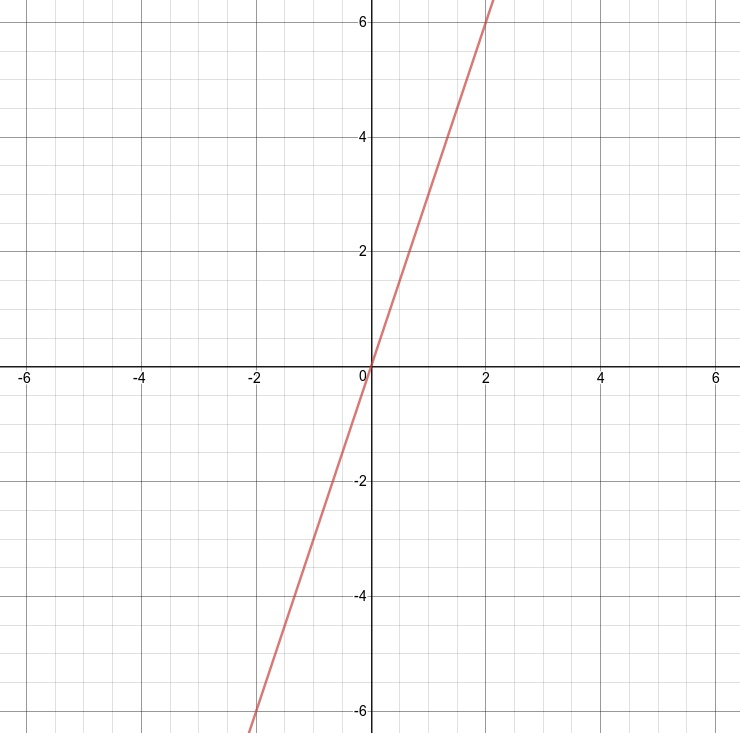
\includegraphics[scale=0.4]{\bank/linearization/figures/line.png}

    
	\sol{
	All three can be linerized about $x=0$ to the function in the graph.



	% TODO: detailed explanation
	}
